\title{Applied $\pi$ calculus}
%\subtitle{}
%\author{Enrico Polesel}
%\institute[Scuola Normale Superiore]{Scuola Normale Superiore}
\date{17 Luglio 2017}

\author{Enrico Polesel}



\begin{frame}[plain]
  \titlepage
\end{frame}

\begin{frame}[plain]
 \frametitle{Indice}
 \tableofcontents
\end{frame}


%\AtBeginSection[]
%{
%  \begin{frame}{\secname}
%    \tableofcontents[currentsection]
%  \end{frame}
%}


\AtBeginSubsection[]
{
  \begin{frame}[plain]{\secname $\rightarrow$ \subsecname}
    \tableofcontents[currentsubsection]
  \end{frame}
}

\section{$\pi$ calcolo e spi calcolo}

\subsection{$\pi$ calcolo}

\begin{frame}
  \frametitle{Sintassi}
  Costruiamo un $\pi$ calcolo che supporti le coppie, ma non
  supportiamo la scelta non deterministica ($P+Q$).

  I termini sono:
  \begin{align*}
    L,M,N,T,U,V & \coloncolonequals & \text{terms} \\
                & a,b,c,\dots,k,\dots,m,n,\dots,s & \text{name} \\
                & x,y,z & \text{variable} \\
                & (M,N) & \text{pair}
  \end{align*}
\end{frame}

\begin{frame}
  I processi sono:
  \begin{align*}
    P,Q,R & \coloncolonequals & \text{plain processes} \\
          & \mathbf{0} & \text{null process} \\
          & P | Q & \text{parallel composition} \\
          & !P & \text{replication} \\
          & \nu n.P & \text{name restriction (new)} \\
          & if\ M=N\ then\ P & \text{conditional} \\
          & N(x).P & \text{message input} \\
          & \obar{N}\left< M\right> .P & \text{message output} \\
          & let\ (x,y) = M\ in\ P & \text{pair splitting}
  \end{align*}
\end{frame}

\begin{frame}{Nomi privati}
  Come nel CCS, possiamo restringere i nomi ad alcuni contesti, ad
  esempio nel processo:
  \begin{align*}
  K(M) = \nu n. \pa{ \obar{n}\ang{M}.\mathbf{0} | n(x).P }
    \onslide<2->{ |C }& &  n\not\in
    fv(P)
  \end{align*}

  esternamente non possiamo osservare il contenuto di $M$ se non per
  gli effetti di $P$, cioè:
  \[ P\bra{\sfrac{M}{x}} \approx P\bra{\sfrac{M'}{x}} \Rightarrow K(M)
    \approx K(M') \]
  
  Oltre alla riservatezza abbiamo anche l'autenticit\`a.
\end{frame}

\begin{frame}
  Ma, a differenza del CCS, i nomi privati possono essere comunicati
  all'esterno (scope extrusion), ad esempio:
  \begin{align*}
    A(M) & = \nu
           c_{AB}. \pa{\obar{c_{AS}}\ang{c_{AB}}. \obar{c_{AB}}\ang{M}}
    \\
    B & = c_{SB}(x). x(y) .P \\
    S & = c_{AS}(x) . \obar{c_{SB}} \ang{x} \\
    Inst(M) & = \nu c_{AS}. \nu c_{SB}. \pa{ A(M) | S | B}
  \end{align*}
  \begin{center}
    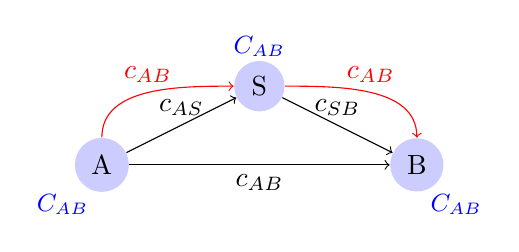
\begin{tikzpicture}[mnode/.style={circle,fill=blue!20}]
      \node[mnode] (A) at (0,0) {A};
      \node[mnode] (S) at (2,1) {S};
      \node[mnode] (B) at (4,0) {B};
      \onslide<2->{\node[blue] (Al) at (-.5,-.5) {\small $C_{AB}$};}
      \onslide<3->{\node[blue] (Sl) at (2,1.5) {\small $C_{AB}$};}
      \onslide<4->{\node[blue] (Bl) at (4.5,-.5) {\small $C_{AB}$};}

      \draw[->] (A) -- node[above] {$c_{AS}$} (S) ;
      \draw[->] (S) -- node[above] {$c_{SB}$} (B) ;
      \onslide<5->{\draw[->] (A) -- node[below] {$c_{AB}$} (B) ;}
      \onslide<3>{\draw[->,red] (A) .. controls +(up:1cm) and +(left:1cm) .. node[above] {$\ang{c_{AB}}$} (S) ;}
      \onslide<4>{\draw[->,red] (S) .. controls +(right:1cm) and +(up:1cm) .. node[above] {$\ang{c_{AB}}$} (B) ;}
%      \draw[->] (A) to [bend left] (S) ;
    \end{tikzpicture}
  \end{center}
\end{frame}

\begin{frame}{Limiti del $\pi$-calcolo}
  Il $\pi$-calcolo ci permette quindi di esprimere
  \begin{itemize}
  \item Segreti condivisi: $\nu k ( A|B)$;
  \item canali ristretti.
  \end{itemize}
  I nostri termini esprimono le coppie. 
  \vfill

  Non abbiamo modi semplici di modellare, ad esempio, una
  comunicazione cifrata (con un segreto condiviso $k$) su un canale
  pubblico.
\end{frame}

\subsection{spi calcolo}

\begin{frame}{Sintassi}
  Consideriamo un'estensione con cifratura simmetrica:
  \begin{align*}
    L,M,N,T,U,V & \coloncolonequals & \text{terms} \\
                & \cdots & \text{vedi precedenti} \\
                & \set{M}_N & \text{codifica}
  \end{align*}
  \begin{align*}
    P,Q,R & \coloncolonequals & \text{plain processes} \\
          & \cdots & \text{vedi precedenti} \\
          & case\ L\; of\; \set{x}_N\ in\ P & \text{decodifica}
  \end{align*}

  Dove
  \[ \pa{ case\ \set{M}_N\; of\; \set{x}_N\ in\ P} \approx
    P\bra{\sfrac{M}{x}} \]
\end{frame}

\begin{frame}{Ipotesi su $\set{M}_N$}
  $\set{M}_N$ pu\`o essere un qualsiasi algoritmo di cifratura simmetrica,
  noi ci limiteremo a chiedere che:
  \begin{itemize}
  \item $\set{M}_N$ si possa decifrare solo conoscendo $N$;
  \item conoscere $\set{M}_N$ e $M$ non sia sufficiente per ricavare $N$;
  \item $\set{M}_N$ contenga abbastanza informazioni per capire se \`e stato
    decifrato con la chiave giusta.
  \end{itemize}
  \vfill
  \pause

  Perdiamo visibilit\`a degli aspetti probabilistici e di
  complessit\`a. Ad esempio non vediamo gli attacchi del compleanno.
\end{frame}

\begin{frame}{Esempio}
  \begin{align*}
    A(M) & = \nu k_{AB}. \pa{
           \obar{c_{AS}}\ang{\set{k_{AB}}_{k_{AS}}}. \obar{c_{AB}}\ang{\set{M}_{k_{AB}}}}
    \\
    S & = c_{AS}(x).case\ x\ of\ \set{y}_{k_{AS}}in\ 
        \obar{c_{SB}}\ang{\set{y}_{k_{SB}}} \\ 
    B & = c_{SB}(x).case\ x\ of\ \set{y}_{k_{SB}}in\ c_{AB}(z). case\
        z\ of\ \set{w}_y in\ P(w) \\ 
    Inst(M) & = \nu k_{AS}. \nu k_{SB}. \pa{ A(M) | S | B } 
  \end{align*}

  %TODO: disegno
  \begin{center}
    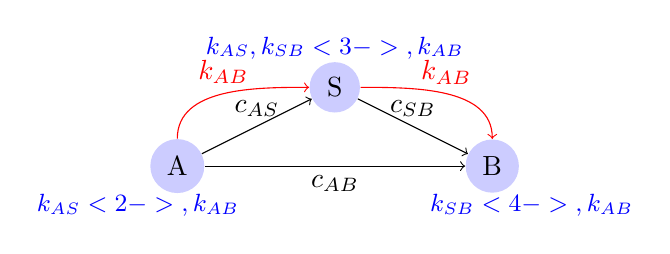
\begin{tikzpicture}[mnode/.style={circle,fill=blue!20}]
      \node[mnode] (A) at (0,0) {A};
      \node[mnode] (S) at (2,1) {S};
      \node[mnode] (B) at (4,0) {B};
      \node[blue] (Al) at (-.5,-.5) {\small $k_{AS}\onslide<2->{, k_{AB}}$};
      \node[blue] (Sl) at (2,1.5) {\small $k_{AS},
        k_{SB}\onslide<3->{, k_{AB}}$};
      \node[blue] (Bl) at (4.5,-.5) {\small $k_{SB}\onslide<4->{, k_{AB}}$};

      \draw[->] (A) -- node[above] {$c_{AS}$} (S) ;
      \draw[->] (S) -- node[above] {$c_{SB}$} (B) ;
      \draw[->] (A) -- node[below] {$c_{AB}$} (B) ;
      \onslide<3>{\draw[->,red] (A) .. controls +(up:1cm) and +(left:1cm) .. node[above] {$\ang{k_{AB}}$} (S) ;}
      \onslide<4>{\draw[->,red] (S) .. controls +(right:1cm) and +(up:1cm) .. node[above] {$\ang{k_{AB}}$} (B) ;}
%      \draw[->] (A) to [bend left] (S) ;
    \end{tikzpicture}
  \end{center}

\end{frame}


\begin{frame}{\textit{Barb}}
  Diciamo che un processo $P$ esibisce un \textit{barb} sul nome
  $\beta \in \set{m,\bar m}$ se il processo comunica su quel nome in
  modo pubblico, cioè
  \begin{align*}
    m(x).P \downarrow m & & \bar m \ang{M}.P \downarrow \bar m 
  \end{align*}
  \begin{align*}
    \frac{P\downarrow \beta}{ P|Q \downarrow \beta} & &
                                                        \frac{P\downarrow
                                                        \beta\; \beta
                                                      \not\in \set{m,
                                                      \bar m}}{ \nu
                                                      m. P \downarrow
                                                      \beta} & & \frac{
                                                               P
                                                               \equiv
                                                               Q \;\; Q
                                                               \downarrow
                                                               \beta}
                                                               {
                                                               P\downarrow
                                                               \beta}
  \end{align*}
  \begin{align*}
    \frac{P\downarrow \beta}{P\Downarrow \beta} & & \frac{P\rightarrow
                                                    Q\;\; Q \Downarrow
                                                    \beta }{P
                                                    \Downarrow \beta}
  \end{align*}
\end{frame}

\begin{frame}{Test}
  Un test è dato da un \textit{barb} $\beta$ e un processo chiuso
  $R$. Diciamo che un processo chiuso $P$ passa il test se $(P|R)
  \Downarrow \beta$.
  \vfill

  \begin{mydef}
    Diciamo che $P \sqsubseteq Q$ se
    $\forall (R,\beta)\;\; (P|R)\Downarrow \beta \Rightarrow
    (Q|R)\Downarrow \beta$.

    Diciamo che $P \simeq Q$ se $P \sqsubseteq Q$ e $Q \sqsubseteq P$.
  \end{mydef}
\end{frame}

\section{Applied $\pi$ calculus}

\subsection{Sintassi}

\begin{frame}{Termini}
  Sia $\Sigma$ una signature di simboli di funzione.  
  \begin{align*}
    L,M,N,T,U,V & \coloncolonequals & \text{terms} \\
                & a,b,c,\dots,k,\dots,m,n,\dots,s & \text{name} \\
                & x,y,z & \text{variable} \\
                & f(M_1,\dots,M_l), f\in \Sigma & \text{function application}
  \end{align*}
  con $l$ opportuno.

  Avremo anche una teoria che ci permetter\`a di scrivere:
  \begin{align*}
    \Sigma \vdash M = N & & \Sigma \not\vdash M = N
  \end{align*}
\end{frame}

\begin{frame}{Processi}
  \begin{align*}
  P,Q,R & \coloncolonequals & \text{plain processes} \\
  & \mathbf{0} & \text{null process} \\
  & P | Q & \text{parallel composition} \\
  & !P & \text{replication} \\
  & \nu n.P & \text{name restriction (new)} \\
  & if\ M=N\ then\ P\ else\ Q & \text{conditional} \\
  & N(x).P & \text{message input} \\
  & \obar{N}\left< M\right> .P & \text{message output}
\end{align*}

\end{frame}

\begin{frame}{Processi estesi}
  \begin{align*}
    A,B,C & \coloncolonequals & \text{extended processes} \\
          & P & \text{plain process} \\
          & A | B & \text{parallel composition} \\
          & \nu n.A & \text{name restriction} \\
          & \nu x.A & \text{variable restriction} \\
          & \left\{ \sfrac{M}{x} \right\} & \text{active substitution}
  \end{align*}
  
  La sostituzione $\left\{ \sfrac{M}{x} \right\}$ \`e pu\`o agire in
  tutti i contesti con cui viene a contatto, per controllare questa cosa
  possiamo mettere una restrizione sulla variabile $\nu x.\left( \left\{
      \sfrac{M}{x} \right\} | P\right)$.
\end{frame}

\begin{frame}{Frame}
  \begin{mydef}[Frame]
    Un processo esteso costituito solo da estensioni attive con
    eventualmente dei nomi ristretti.
  \end{mydef}
  \[ \nu \tilde n = \nu n_1. \dots \nu n_k \]
  \[ \sigma = \set{ \sfrac{\tilde M}{\tilde x}} = \set{
      \sfrac{M_1}{x_1}, \dots \sfrac{M_l}{x_l}} = \set{
      \sfrac{M_1}{x_1}}| \cdots | \set{\sfrac{M_l}{x_l}} \]
  \[ \varphi = \nu n_1.\nu n_2.\dots \nu n_k . \pa{ \set{
        \sfrac{M_1}{x_1}}| \cdots | \set{\sfrac{M_l}{x_l}}} = \nu
    \tilde n. \sigma \]
  \vfill

  Dato un processo esteso $A$ posso rimuovere tutto ci\`o che non \`e
  una sostituzione attiva o un nome ristretto ottenendo il
  \textbf{comportamento statico} $\varphi(A)$.
\end{frame}

\begin{frame}{Free variables e free names}
  \begin{align*}
    fv(x) & \eqdef \set{x} & fn(x) & \eqdef \emptyset \\
    fv(n) & \eqdef \emptyset &  fn(n) & \eqdef \set{n} \\
    fv\pa{f\pa{ M_1, \dots }} & \eqdef fv\pa{M_1} \cup \cdots  & fn(f(...)) & \eqdef ... \\
          & \vdots & &\vdots  \\
    fv(N(x).P) & \eqdef fv(N) \cup \pa{fv(P) \setminus \set{x}} &   fn(N(x).P) & \eqdef fn(N) \cup fn(P) \\
          & \vdots & & \vdots \\
    fv(\nu x.A) & \eqdef fv(A) \setminus \set{x} &   fn(\nu n.P) & \eqdef fn(P)\setminus \set{n} \\
    fv\pa{ \set{ \sfrac{M}{x} } } & \eqdef fv(M) \cup \set{x} & fn\pa{ \set{ \sfrac{M}{x} } } & \eqdef fn(M) \\
  \end{align*}
\end{frame}

\begin{frame}{Dominio di un processo esteso}
  \begin{align*}
    dom(P) & \eqdef \emptyset \\
    dom(A|B) & \eqdef dom(A) \cup dom(B) \\
    dom(\nu n.A) & \eqdef dom(A) \\
    dom(\nu x.A) & \eqdef dom(A) \setminus \set{x}\\
    dom\pa{ \set{ \sfrac{M}{x}}} & \eqdef \set{x}           
  \end{align*}
  \vfill
  
  Diciamo che un processo esteso $A$ \`e chiuso se $fv(A) = dom(A)$.
\end{frame}

\subsection{Semantica}

\begin{frame}{Contesti}
  Un contesto $E[\_]$ \`e un'espressione con un argomento.
  \begin{mydef}[Contesto di valutazione]
    Un contesto di valutazione \`e un contesto il cui argomento non
    \`e sottoposto a replicazione, condizionale, input o output.
  \end{mydef}
  \begin{mydef}[Contesto chiuso]
    Il contesto $E[\_]$ chiude $A$ se $E[A]$ \`e chiuso.
  \end{mydef}
\end{frame}


\begin{frame}{Equivalenza strutturale}
  \begin{align*}
    A & \equiv A|\mathbf{0} & A|(B|C) & \equiv (A|B)|C \\
    A|B & \equiv B|A & !P & \equiv P|!P \\ \\
    \nu n.\mathbf{0} & \equiv \mathbf{0} & \nu u. \nu v.A & \equiv \nu v. \nu
                                                   u.A \\
    A| \nu u.B & \equiv \nu u. (A|B) & \text{when } & u\not\in fv(A)
                                                     \cup fn(A) \\ \\
    \nu x. \set{\sfrac{M}{x}} & \equiv \mathbf{0} & \set{\sfrac{M}{x}}
                                                    |A & \equiv
                                                         \set{\sfrac{M}{x}}
                                                         |
                                                         A\bra{\sfrac{M}{x}}
    \\
    \set{\sfrac{M}{x}} & \equiv \set{\sfrac{N}{x}} & \text{when } &
                                                                   \Sigma
                                                                   \vdash M=N
  \end{align*}
\end{frame}

\begin{frame}
  Usando l'equivalenza strutturale possiamo riscrivere ogni processo
  esteso chiuso come:
  \[ A \equiv \nu \tilde n. \pa{ \set{\sfrac{\tilde M}{\tilde x}} | P
    } \]
  dove $P$ \`e un processo, $fv(P)\ = \emptyset$, $fv(\tilde M) =
  \emptyset$ e $\set{\tilde n} \subseteq fn(\tilde M)$.
  \vfill

  Per ogni frame $\varphi$ chiuso:
  \[ \varphi \equiv \nu \tilde n. \set{\sfrac{\tilde M}{\tilde x}} \]
\end{frame}

\begin{frame}{Internal reduction}
  Consideriamo la pi\`u piccola relazione sui processi estesi chiusa
  per equivalenza strutturale e applicazione di contesti di
  valutazione tale che:
  \begin{align*}
    \obar{N}\ang{x}.P|N(x).Q & \rightarrow P|Q \\
    if\ M=M\ then\ P\ else\ Q & \rightarrow P \\
    if\ M=N\ then\ P\ else\ Q & \rightarrow Q \\
  \end{align*}
\end{frame}

\begin{frame}
    Ad esempio se $x \not\in fv(N)\cup fv(M)\cup fv(P)$:
  \begin{align*}
    \obar{N}\ang{M}.P | N(x).Q & \equiv \nu x. \pa{ \set{\sfrac{M}{x}} } | \obar{N}\ang{M}.P | N(x).Q \\
    & \equiv \nu x. \pa{ \set{\sfrac{M}{x}} | \obar{N}\ang{M}.P | N(x).Q }\\
    & \equiv \nu x.\pa{ \set{\sfrac{M}{x}} | \obar{N} \ang{x}.P | N(x).Q } \\
    & \rightarrow \nu x.\pa{\set{\sfrac{M}{x}}|P|Q} \\
    & \equiv \nu x.\pa{\set{\sfrac{M}{x}}|P|Q\bra{\sfrac{M}{x}}} \\
    & \equiv \nu x.\pa{\set{\sfrac{M}{x}}}|P|Q\bra{\sfrac{M}{x}} \\
    & \equiv P|Q\bra{\sfrac{M}{x}}
  \end{align*}
\end{frame}

\subsection{Esempi}

\begin{frame}{Coppie}
  % \begin{align*}
  %   \mathrm{zero} &: \mathrm{Data} \\
  %   \mathrm{suc} &: \mathrm{Data} \rightarrow \mathrm{Data} \\
  %   \mathrm{prev} &: \mathrm{Data} \rightarrow \mathrm{Data}
  % \end{align*}
  % Con assiomi: \( \mathrm{prev} \pa{ \mathrm{suc} (x) } = x, \dots \)
  % \vfill
  
  \begin{align*}
    \mathrm{pair} &: \mathrm{Data} \times \mathrm{Data} \rightarrow
                    \mathrm{Data} \\
    \mathrm{fst} &: \mathrm{Data} \rightarrow \mathrm{Data} \\
    \mathrm{snd} &: \mathrm{Data} \rightarrow \mathrm{Data}
  \end{align*}
  Con:
  \begin{itemize}
  \item $\mathrm{fst}\pa{\mathrm{pair}(x,y)} = x$,
  \item $\mathrm{snd}\pa{\mathrm{pair}(x,y)} = y$.
  \end{itemize}

\end{frame}

\begin{frame}{Funzioni hash}
  Una funzione hash \`e una funzione $\mathrm{h}: \mathrm{Data}
  \rightarrow \mathrm{Data}$ senza equazioni.
  
  \begin{align*}
    A & \;=\; \obar{a}\ang{ \pa{M,\mathrm{h}\pa{(k,M)}}} \\
    B & \;=\; a(x).if\ \mathrm{h}\pa{(k,\mathrm{fst}(x))} =
        \mathrm{snd}(x)\ then\ \obar{b}\ang{\mathrm{fst}(x)} \\
    Inst & \;=\; \nu k.\pa{ A | B } 
  \end{align*}
\end{frame}

\begin{frame}{Cifratura simmetrica}
  Abbiamo due funzioni
  \begin{align*}
    \mathrm{enc} &: \mathrm{Data} \times \mathrm{Data} \rightarrow
                   \mathrm{Data} \\
    \mathrm{dec} &: \mathrm{Data} \times \mathrm{Data} \rightarrow
                   \mathrm{Data} \\
  \end{align*}
  tali che $\mathrm{dec}\pa{\mathrm{enc}(x,y),y} = x$ dove $x$
  rappresenta il testo in chiaro e $y$ la chiave.
  \vfill
  
  \begin{align*}
    A & \;=\; \obar{a}\ang{\mathrm{enc}(M,k)} \\
    B & \;=\; a\pa{x}.if\ \mathrm{enc}\pa{ \mathrm{dec}(x,k)} =
        x\ then\ \obar{b}\ang{\mathrm{dec}(x,k)} \\
    Inst & \;=\; \nu k. \pa{ A|B}
  \end{align*}
\end{frame}

\begin{frame}{Cifratura asimmetrica}
  Usiamo quattro funzioni $\mathrm{enc}$, $\mathrm{dec}$,
  $\mathrm{pk}$ e $\mathrm{sk}$ tali che
  \[ \mathrm{dec}\pa{\mathrm{enc}\pa{x,\mathrm{pk}(y)},\mathrm{sk}(y)}
    = x \]
  \begin{align*}
    A &= \nu s.\pa{ \obar{a}\ang{\mathrm{pk}(s)}|
    b(x).\obar{c}\ang{\mathrm{dec}\pa{ x,\mathrm{sk}(s) } } } \\
    B &= a(y).\obar{b}\ang{\mathrm{enc}(M,y)} \\
    C &= A|B   
  \end{align*}
  \vfill
  \onslide<2->{
  Potremmo chiedere altre propriet\`a, ad esempio:
  \[ \mathrm{dec}\pa{\mathrm{enc}(x,y),z} =
    \mathrm{enc}\pa{\mathrm{dec}(x,y),y} \]}
\end{frame}

\section{Equivalenze}

\subsection{Osservazionale}

\begin{frame}{Definizione}
  Scriviamo $A \Downarrow a$ quando $A$ pu\`o inviare un messaggio sul
  nome $a$, cio\`e esiste $E$ contesto di valutazione che non lega $a$
  tale che:
  \[ A \rightarrow ^* E\bra{ \obar{a}\ang{M}.P} \]

  \begin{mydef}[Equivalenza osservazionale]
    Una bisimulazione osservazionale \`e una relazione simmetrica
    $\mathcal{R}$ tra processi estesi chiusi sullo stesso dominio tale
    che $A \mathcal{R} B$ implica:
    \begin{enumerate}
    \item $A \Downarrow a \Rightarrow B \Downarrow a$;
    \item se $A \rightarrow ^* A'$ con $A'$ chiuso allora $\exists B'$
      t.c. $B \rightarrow ^* B'$ e $A' \mathcal{R} B'$;
    \item $\forall E[\_]$ contesto di valutazione chiuso $E[A]
      \mathcal{R} E[B]$.
    \end{enumerate}
    Chiamiamo \textbf{equivalenza osservazionale} ($\approx$) la pi\`u
    grande bisimulazione osservazionale.
  \end{mydef}
\end{frame}

\begin{frame}{Esempio}
  Se $h$ \`e una funzione senza equazioni (ad esempio una funzione
  hash) allora
  \[ \nu s. \obar{a}\ang{s} \approx \nu s. \obar{a}\ang{h(s)} \]
\end{frame}

\subsection{Statica}

\begin{frame}
  Ci concentriamo sui frame, abbiamo gi\`a visto che ad ogni processo
  esteso $A$ possiamo associare il suo frame $\varphi (A)$.
  \vfill
  
  Siano $f$, $g$ due funzioni senza equazioni:
  \begin{align*}
    \varphi _0 &= \nu k.\set{\sfrac{k}{x}} | \nu s. \set{\sfrac{s}{y}}
    \\
    \varphi _1 &= \nu k.\set{ \sfrac{f(k)}{x}, \sfrac{g(k)}{y}} \\
    \varphi _2 &= \nu k.\set{ \sfrac{k}{x}, \sfrac{f(k)}{y}} 
  \end{align*}
  Un contesto non pu\`o distinguere fra $\varphi _0$ e $\varphi _1$,
  mentre $\varphi _2$ pu\`o essere distinto dagl'altri testando il
  predicato $f(x) = y$.
  \[ \varphi _0 \approx _s \varphi _1 \not \approx _s \varphi _2 \]
\end{frame}

\begin{frame}
  \begin{mydef}[Uguaglianza di termini in un frame]
    $(M=N)\varphi$ se e solo se esistono $\tilde n$ e $\sigma$ tali che:
    \begin{itemize}
    \item $fv(M) \cup fv(N) \subseteq dom(\varphi)$;
    \item $\varphi \equiv \nu \tilde n.\sigma$;
    \item $\set{\tilde n} \cap( fn(M) \cup fn(N)) = \emptyset$;
    \item $M\sigma = N\sigma$.
    \end{itemize}
  \end{mydef}
  \vfill
  
  Nei frame precedenti:
  \begin{align*}
    (f(x) \neq y)\varphi _0 && (f(x) \neq y)\varphi _1 && (f(x) =
                                                        y)\varphi _2
  \end{align*}
\end{frame}

\begin{frame}{Definizione}
  \begin{mydef}[Equivalenza di frame]
    Due frame chiusi $\varphi, \psi$ sono staticamente equivalenti
    ($\varphi \approx _s \psi$) se
    \begin{itemize}
    \item $dom(\varphi) = dom(\psi)$
    \item $\forall M,N\; (M=N)\varphi \Leftrightarrow (M=N)\psi$
    \end{itemize}
  \end{mydef}

  \begin{mydef}[Equivalenza di processi estesi]
    Due processi estesi chiusi $A,B$ sono staticamente equivalente
    ($A \approx_s B$) se e solo se i loro frame sono staticamente
    equivalenti:
    \[ A \approx _s B \Leftrightarrow \varphi(A) \approx _s \varphi(B) \]
  \end{mydef}
\end{frame}

\begin{frame}
  \begin{mylem}
    Siano $A$, $B$ processi estesi chiusi.
    \begin{itemize}
    \item se $A \equiv B$ o $A \rightarrow B$ allora $A \approx _s B$;
    \item se $A \approx _s B$ allora per ogni contesto di valutazione
      chiuso $E[\_]$ si ha $E[A] \approx _s E[B]$.
    \end{itemize}
  \end{mylem}
  \vfill
  
  \begin{mylem}
    L'equivalenza osservazionale coincide con l'equivalenza statica
    sui frame
    \[ \varphi \approx \psi \Leftrightarrow \varphi \approx _s \psi \]
  \end{mylem}
  \pause 
  \[ (M=N)\varphi \Leftrightarrow \pa{ \varphi | if\ N=M\ then\
      \obar{a}\ang{n}} \Downarrow a \]
\end{frame}
\begin{frame}{Relazione con l'equivalenza osservazionale}
  \begin{mypro}
    L'equivalenza osservazionale \`e strettamente pi\`u fine
    dell'equivalenza statica $\approx \subset \approx _s$
    \[ A \approx B \Rightarrow A \approx _s B \]
  \end{mypro}
  \vfill

  \begin{align*}
    A &= \obar{a}\ang{n} & A &\not\approx B \\
    B &= \obar{b}\ang{n} & A &\approx _s B 
  \end{align*}
\end{frame}

\subsection{Etichettata}

\begin{frame}{Semantica etichettata}
  Oltre alla riduzione $\rightarrow$ aggiungiamo una nuova relazione
  $\xrightarrow{\alpha}$ dove $\alpha$ pu\`o essere:
  \begin{itemize}
  \item $N(M)$: l'input di $M$ sul canale $N$;
  \item $\nu x.\obar{N}\ang{x}$ (con $x\not\in fv(N)$): l'output di
    $x$ su $N$.
  \end{itemize}
  
  Le principali regole sono:
  \begin{itemize}
  \item In: \( N(x).P \xrightarrow{N(M)} P\bra{\sfrac{M}{x}} \)
  \item Out-Var \( \displaystyle \frac{x\not\in
      fv\pa{\obar{N}\ang{M}.P}}{\obar{N}\ang{M}.P \xrightarrow{\nu
        x.\obar{N}\ang{x}} P|\set{\sfrac{M}{x}}} \)
  \end{itemize}

\end{frame}

\begin{frame}
  Abbiamo altre regole per gestire lo scoping:
  \[ \frac{A \xrightarrow{\alpha} A'\; u\not\in\alpha}{\nu u.A
      \xrightarrow{\alpha} \nu u.A'} \]
  il parallelismo:
  \[ \frac{A \xrightarrow{\alpha} A'\;bv(\alpha) \cap fv(B) =
      \emptyset}{A|B \xrightarrow{\alpha} A'|B} \]
  e l'equivalenza strutturale:
  \[ \frac{A \equiv B\;\; B\xrightarrow{\alpha} B'\;\; B' \equiv A'}{A
      \xrightarrow{\alpha} A'} \]
\end{frame}

\begin{frame}{Esempio}
  \begin{align*}
    & \nu k. \obar{a} \ang{\mathrm{enc}(M,k)}.\obar{a}\ang{k}.a(z).if\
      z=M\ then\ \obar{c}\ang{n} \\
    \xrightarrow{\nu x.\obar{a}\ang{x}} & \nu
                                          k.\pa{\set{\sfrac{\mathrm{enc}(M,k)}{x}}|
                                          \obar{a}\ang{k}. a(z).if\
                                          z=M\ then\ \obar{c}\ang{n}}
    \\
    \xrightarrow{\nu y.\obar{a}\ang{y}} & \nu k. \pa{
                                          \set{\sfrac{\mathrm{enc}(M,k)}{x}}
                                          | \set{\sfrac{k}{y}} |
                                          a(z).if\ z=M\ then\
                                          \obar{c}\ang{n}} \\
    \xrightarrow{a\pa{\mathrm{dec}(x,y)}} & \nu k. \pa{
                                            \set{\sfrac{\mathrm{enc}(M,k)}{x}}
                                            | \set{\sfrac{k}{y}} | if\
                                            \mathrm{dec(x,y)}=M\ then\
                                            \obar{c}\ang{n}} \\
    \rightarrow & \nu k. \pa{ \set{\sfrac{\mathrm{enc}(M,k)}{x}} |
                  \set{\sfrac{k}{y}} | \obar{c}\ang{n}} 
  \end{align*}
\end{frame}

\begin{frame}{Definizione}
  \begin{mydef}[Equivalenza etichettata]
    Una \textbf{bisimulazione etichettata} \`e una relazione
    simmetrica $\mathcal{R}$ sui processi estesi chiusi tale che $A
    \mathcal{R} B$ implica:
    \begin{enumerate}
    \item $A \approx _s B$;
    \item se $A \rightarrow A'$ con $A'$ chiuso allora esiste $B'$
      chiuso tale che $B \rightarrow ^* B'$ e $A' \mathcal{R} B'$;
    \item se $A \xrightarrow{\alpha} A'$ con $A'$ chiuso e
      $fv(\alpha) \subseteq dom(A)$ allora esiste $B'$ tale che
      $B \rightarrow ^* \xrightarrow{\alpha} \rightarrow ^* B'$ e
      $A' \mathcal{R} B'$.
    \end{enumerate}
    L'\textbf{equivalenza etichettata} (o bisimilarit\`a etichettata)
    $\approx _l$ \`e la pi\`u grande bisimulazione etichettata.
  \end{mydef}
\end{frame}

\begin{frame}{Relazione con l'equivalenza osservazionale}
  \begin{myteo}
    L'equivalenza osservazionale coincide l'equivalenza etichettata
    \[ \approx = \approx _l \]
  \end{myteo}
\end{frame}

\section{Esempio}

\subsection{Diffie-Hellman Key Agreement}

\begin{frame}{Funzioni}
  Prendiamo due simboli di funzione $f$ (che prende due argomenti) e
  $g$ (che prene un argomento) tali che
  \[ f\pa{x,g(y)} = f\pa{g(x),y} \]
  \vfill

  Vogliamo far parlare due partecipanti $A_0$ e $A_1$, per
  semplicit\`a usiamo due canali monodirezionali $c_{01}$ e $c_{10}$,
  vogliamo stabilire una chiave condivisa segreta $y$ da far
  utilizzare a due processi $P_0$ e $P_1$.
\end{frame}

\begin{frame}
  \begin{align*}
    \onslide<2->{x_0 &= g(n_0) & x_1 &=g(n_1)}
  \end{align*}
  \[ \onslide<3->{y_0 = f(n_0,x_1) = f(n_0,g(n_1)) = f(g(n_0),n_1) = g(x_0,n_1) =
    y_1} \]
  \begin{align*}
    \onslide<2->{\sigma _0 & \eqdef \set{\sfrac{g(n_0)}{x_0}} & \sigma _1 & \eqdef
                                                               \set{\sfrac{g(n_1)}{x_1}}
    \\ }
    \onslide<3->{\phi _0 & \eqdef \set{\sfrac{f(n_0,x_1)}{y}} & \phi _1 & \eqdef
                                                             \set{\sfrac{
                                                             f(x_0,n_1)}{y}} }
  \end{align*}
  \begin{align*}
    A_0 &= \nu n_0.\pa{ \obar{c_{01}}\ang{x_0\sigma _0} |
          c_{10}(x_1).P_0\phi _0 } \\
    A_1 &= \nu n_1.\pa{ \obar{c_{10}}\ang{x_1\sigma _1} |
          c_{01}(x_0).P_1\phi _1 }
  \end{align*}
  \begin{center}
    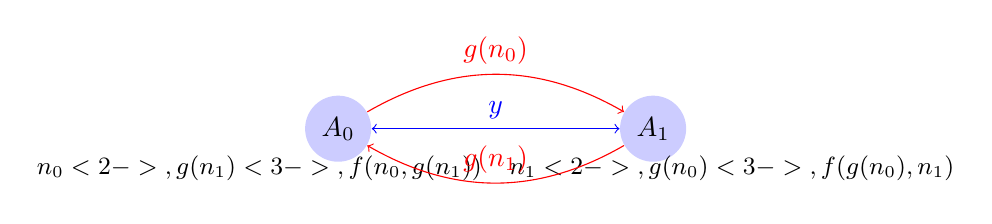
\begin{tikzpicture}[mnode/.style={circle,fill=blue!20}]
      \node[mnode] (A0) at (0,0) {$A_0$};
      \node[mnode] (A1) at (4,0) {$A_1$};
      
      \node (l0) at (-1,-.5) {\small $n_0\onslide<2->{,
          g(n_1)}\onslide<3->{, f(n_0,g(n_1))}$} ;
      \node (l1) at (5,-.5) {\small $n_1\onslide<2->{,
          g(n_0)}\onslide<3->{, f(g(n_0),n_1)}$} ;
      
      \onslide<2>{\draw[->,red] (A0) to [bend left] node[above] {$g(n_0)$} (A1);}
      \onslide<2>{\draw[->,red] (A1) to [bend left] node[above]
        {$g(n_1)$} (A0);}
      \onslide<3->{\draw[<->,blue] (A0) to node [above] {$y$} (A1) ;}
    \end{tikzpicture}
  \end{center}

\end{frame}

\begin{frame}
    \begin{align*}
    \sigma _0 & \eqdef \set{\sfrac{g(n_0)}{x_0}} & \phi _0 & \eqdef
                                                             \set{\sfrac{
                                                             f(n_0,x_1)}{y}} \\
    \sigma _1 & \eqdef \set{\sfrac{g(n_1)}{x_1}} & \phi _1 & \eqdef
                                                             \set{\sfrac{
                                                             f(x_0,n_1)}{y}} 
  \end{align*}
  \begin{align*}
    A_0 &= \nu n_0.\pa{ \obar{c_{01}}\ang{x_0\sigma _0} |
          c_{10}(x_1).P_0\phi _0 } \\
    A_1 &= \nu n_1.\pa{ \obar{c_{10}}\ang{x_1\sigma _1} |
          c_{01}(x_0).P_1\phi _1 }
  \end{align*}
  L'esecuzione di $A_0|A_1$ porta a:
  \begin{align*}
    A_0 | A_1 \rightarrow ^* \;& \nu x_0.\nu x_1.\nu n_0.\nu
                            n_1.\pa{ P_0 \phi _0 | P_1 \phi _1 |
                            \sigma _0 | \sigma _1 } \\
     \equiv \; &\nu x_0.\nu x_1.\nu n_0.\nu n_1.\nu y.\pa{ P_0 | P_1 |
      \phi _0 | \sigma _0 | \sigma _1 } \\
    \equiv \; & \nu y.\pa{ P_0| P_1 | \nu x_0. \nu x_1. \varphi }
  \end{align*}
  \[ \varphi \eqdef \pa{ \nu n_0.\pa{ \phi _0 | \sigma _0}} | \pa{ \nu
      n_1 . \sigma _1 } \]
\end{frame}

\begin{frame}
  \[ \varphi \eqdef \pa{ \nu n_0.\pa{ \phi _0 | \sigma _0}} | \pa{ \nu
      n_1 . \sigma _1 } \]
  \[ A_0|A_1 \rightarrow ^* \nu y.\pa{ P_0| P_1 | \nu x_0. \nu x_1. \varphi } \]
  Supponiamo che un attaccante possa leggere i messaggi dei canali
  $c_{01}$ e $c_{10}$ ma non li possa modificare, avr\`a quindi
  accesso alle variabili $x_0$ e $x_1$, il nostro processo quindi
  diventa:
  \[ \nu y.\pa{ P_0| P_1 | \varphi } \]
  D'altra parte noi vorremmo che il valore di $y$ fosse riservato,
  cio\`e vorremmo l'equivalenza con il processo:
  \[ \nu k.\pa{P_0|P_1}\bra{\sfrac{k}{y}} \]
\end{frame}

\begin{frame}
  \begin{mypro}
    Siano $P_0$ e $P_1$ due processi con $y$ variabile libera e dove non
    appare il nome $k$, allora:
    \[ \nu y.\pa{ P_0 | P_1 | \varphi } \approx \nu k.\pa{ P_0|P_1 }
        \bra{\sfrac{k}{y}} | \nu s_0. \set{\sfrac{s_0}{x_0}} | \nu
      s_1.\set{\sfrac{s_1}{x_1}} \]
  \end{mypro}
  
  Si pu\`o dimostrare che
  \[ \varphi \approx _s \nu s_0.\nu s_1.\nu k.\set{\sfrac{s_0}{x_0},
      \sfrac{s_1}{x_1}, \sfrac{k}{y}} \]
  Trattandosi di frame l'equivalenza statica si traduce in equivalenza
  osservazionale.

  L'equivalenza osservazionale si mantiene applicando il contesto $\nu
  y.\pa{ P_0 | P_1 | \_ }$.
\end{frame}
